\documentclass{article}
\usepackage[spanish]{babel}
\usepackage{graphicx} % Required for inserting images
\usepackage{float}

\title{\textbf{Receta para hacer roles de canela}}
\author{Tania Paola López Navarro}
\date{27 de septiembre de 2026}

\begin{document}

\maketitle

\section*{Ingredientes}
 \begin{itemize}
     \item Para los rollos
     \begin{enumerate}
        \item 450g de harina
        \item 2 cdta de levadura seca (12 grs aprox)
        \item2 cdas de agua tibia
        \item250 ml de leche tibia
        \item100 g de azúcar blanca
        \item 1 huevo
        \item cdta de Sal de Mar 
        \item 1/4 cdta de Sal de Mar
        \item85 g de mantequilla sin sal
        \item1/2  cdta de Esencia de Vainilla (opcional)
     \end{enumerate}

     \item Para el relleno
     \begin{enumerate}
         \item 70g de mantequilla
         \item 180g de azúcar
         \item 3 cdas de canela molida
     \end{enumerate}
          
 \end{itemize}

 \section{Preparación}
 En un bowl, pon la levadura junto con la leche tibia y el agua tibia, y mezcla. Luego, agrega el azúcar y mezcla bien. Incorpora el huevo batido (con tenedor) y mezcla hasta integrar. \textit{\textbf{Opcionalmente, añade 1/2 cdta de esencia de vainilla.
 }}
 
 Agrega la mitad de la harina y mezcla con movimientos envolventes. Luego, incorpora la mantequilla derretida y finalmente la otra mitad de la harina, junto con la sal. Mezcla bien hasta formar una masa pegajosa, pero \textit{que se despegue del bowl}. 
 
 Deja reposar tapado durante 1 1/2 hora, o hasta que doble su volumen.
 Pon la masa sobre una superficie plana ligeramente enharinada y estírala con un uslero hasta formar \textbf{un rectángulo.}

 \begin{figure}[H]
     \centering
     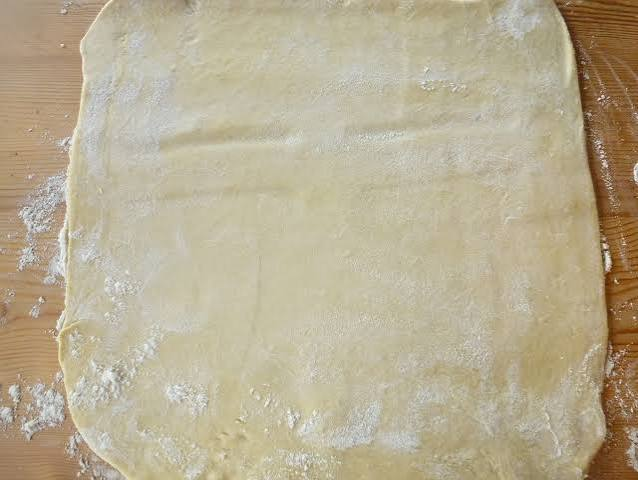
\includegraphics[width=0.50\linewidth]{masa.jpeg}
     \caption{Ejemplo sobre como debe verse la masa}
     \label{fig:placeholder}
 \end{figure}

Para seguir se tiene que hacer el relleno para este sigue los siguientes pasos: Derrite la mantequilla y agrega azúcar morena y canela molida. 

Pincela la masa con esta mezcla por toda la superficie. Luego, enrolla por el lado más largo y córtala en rollos de 1 1/2 a 2 cm aprox.

Coloca los rollos en una lata de horno o fuente enmantequillada, dejando espacio entre cada uno. Deja reposar por al menos 20 minutos, o hasta que dupliquen su tamaño.
Lleva a horno precalentado a 180 °C por 20 minutos.

\begin{figure}[H]
    \centering
    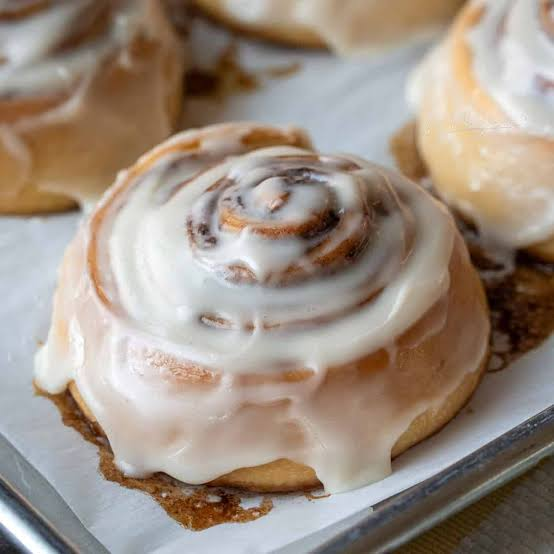
\includegraphics[width=0.50\linewidth]{rolCanela.jpeg}
    \caption{Rol de Canela terminado}
    \label{fig:placeholder}
\end{figure}

\end{document}
